Similar to the JL-Lemma, 
oblivious subspace embeddings (OSEs), are  oblivious, $\epsilon$-distortion, random embeddings.
However, rather than just embedding a finite set of $k$ vectors,
they are concerned with embedding an entire $d$-dimensional subspace. 
In the main work that we covered, \cite{cohen2016nearly}, OSEs are defined as follows:
%
\begin{definition}[Oblivious Subspace Embedding]
    A probability distribution over $m$ by $n$ matrices, $\Pi$,
    is defined to be a $(d, \epsilon, \delta)$-OSE if,
    for any $d$-dimensional subspace $S$ of $\rea^n$,
    \begin{align}
        \pr \left[ \left( \max_{\xx \in S, \norm{x}=1} \left| \norm{\Pi\xx}^2 - 1\right| \right) > \epsilon \right] < \delta.
    \end{align}
\end{definition}
%
From what we've found, 
the extension of the JL-Lemma to subspaces was originally done by~\cite{sarlos2006improved},
who showed that a $d$-dimensional \textit{subspace} of $\rea^n$,
could be embedded into $m=\calO(\epsilon^{-2}d\log(d/\epsilon))$ dimensions
and similarly approximately preserve the lengths of all vectors in the subspace.
The allowable distortion is visualized in Figure~\ref{fig:distortion_and_net} (left).
%
\begin{lemma}
\label{lem:subspace_ext}
Let $S$ be an arbitrary d dimensional subspace of $\rea^n$ and $\epsilon \in (0, 1/2]$, $\delta < 1$. 
If $\Pi$ is a JL transform from $\rea^n$ to 
$m=\calO(\epsilon^{-2}d\log(d/\epsilon) \cdot f(\delta))$ dimensions for some 
function f, then
\begin{align*}
    \pr \left[ \forall \xx \in S~~(1-\epsilon) \norm{\xx} \leq \norm{\Pi\xx} \leq (1+\epsilon)\norm{\xx} \right]
            \geq 1-\delta.
\end{align*}
\end{lemma}
%
\begin{proofsketch}
The key idea of the proof is then to cover the unit sphere with an epsilon-net 
that is sufficiently fine that every $\xx \in S$ is close enough to a point in the net.
This is visualized in Figure~\ref{fig:distortion_and_net}(right).
The epsilon net used in the proof has $\calO((k/\epsilon)^k)$ elements.
Plugging that many elements into the union bound used to prove \ref{thm:jl_lemma},
in place of $\binom{k}{2}$, we get to the stated complexity. 
For more details, see Lemma 10 in \cite{sarlos2006improved}.
\end{proofsketch}
%
\begin{figure}
    \centering
    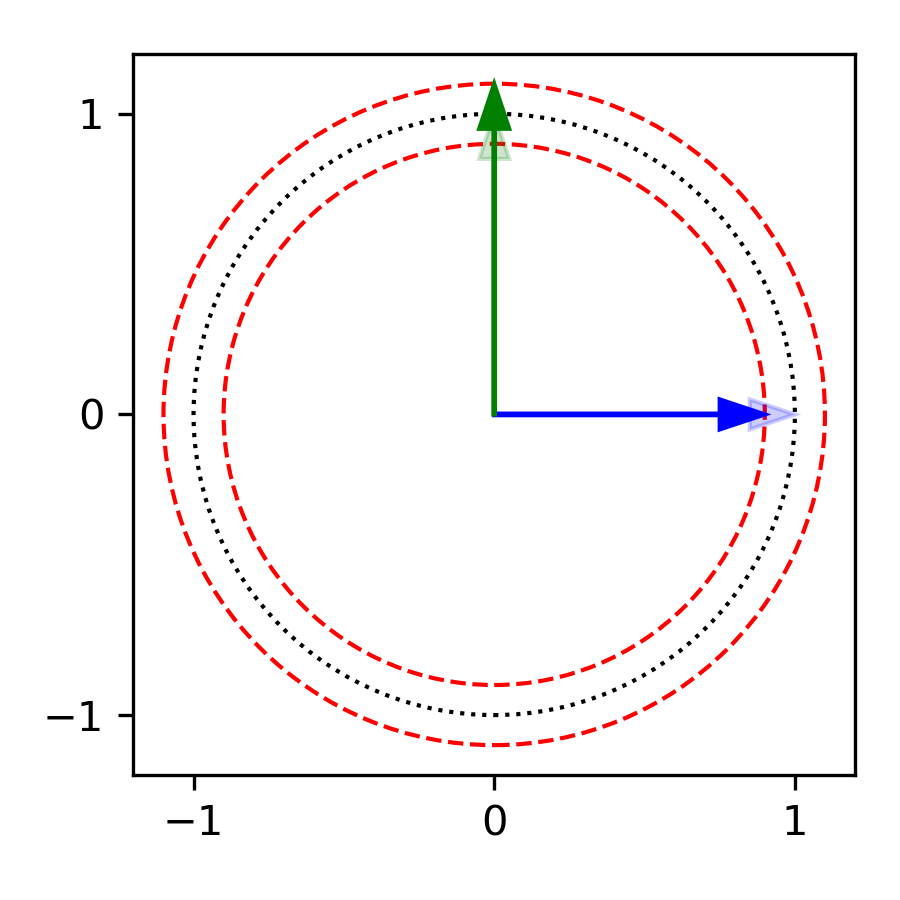
\includegraphics{figures/unit_sphere.png}
    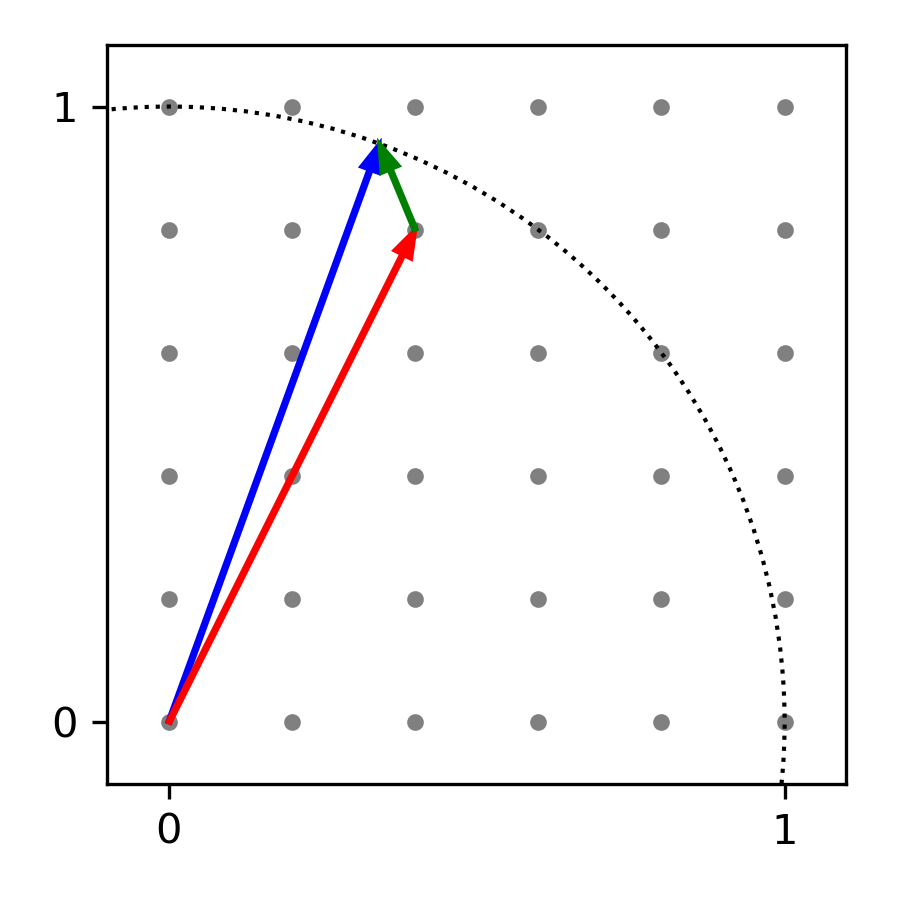
\includegraphics{figures/epsilon_net.png}
    \caption{Left – Visualization of allowable distortion vectors in the preserved subspace $S$. 
    Unit vectors must not be distorted out of the $\pm \epsilon$ shell. 
    Right – Visualization of the epsilon net used to prove Lemma~\ref{lem:subspace_ext}. 
    The blue vector is an arbitary vector on the unit sphere. 
    Using the triangle inequality, its magnitude is less than the sum of the red and green vectors.
    Bounding the distortion of the red vector is easy,
    since it is an element of the net. 
    The distortion of the green vector requires a little more work, 
    but with a sufficiently fine net, this component is very small,
    and the sum of their distortions are shown to be within the $(1\pm \epsilon)$ tolerance. 
    }
    \label{fig:distortion_and_net}
\end{figure}
